\documentclass[12pt]{article}
\usepackage{graphicx}
\usepackage{float}
\usepackage{amsmath}
\usepackage{url}

\restylefloat{figure}
	\title{IT3708 - Exercise 4}
\author{
        Eirik Hammerstad \& Nicklas Utgaard
}

\newcommand{\shiftline}[0]{\hfill\newline\noindent}

\date{\today}
\begin{document}
\maketitle
\section{Disclaimer}
In order to keep to our tradition of using Java in this course we decided to use it to implement our control system during this project. 
Further is it worth noting that we completed this project with three main iterations, each consisting of several subiterations. 

\shiftline The first iteration was used to implement the general architecture as well as the three submodules, 
	\textit{Search}, \textit{Retrieval}, and \textit{Stagnation}, in a very rudemental way.

\shiftline This formed the basis for our second iteration where we converted the provided \textit{C} modules to Java, 
	and introduced \textit{OOP} into these in order to fit into the overall architecture.

\shiftline 	The last iteration of this project was used to identify improvement potential and improve upon these in the three modules implemented during the second iteration.

\section{Part A}
	\subsection{System overview}
		\subsubsection{Architectural description}
			Figure~\ref{fig:architecture} shows the architecture as was at the end of the project. 
			Arrows to packages indicating the usage of all part in that package. 
			E.g \textit{SensoryInput} has an aggregation arrow to the \textit{input} package, which in term indicates that it is an aggregation 
			of the package's internal classes (\textit{LightArray} and \textit{ProximityArray}).
			
			\begin{figure}[H]
				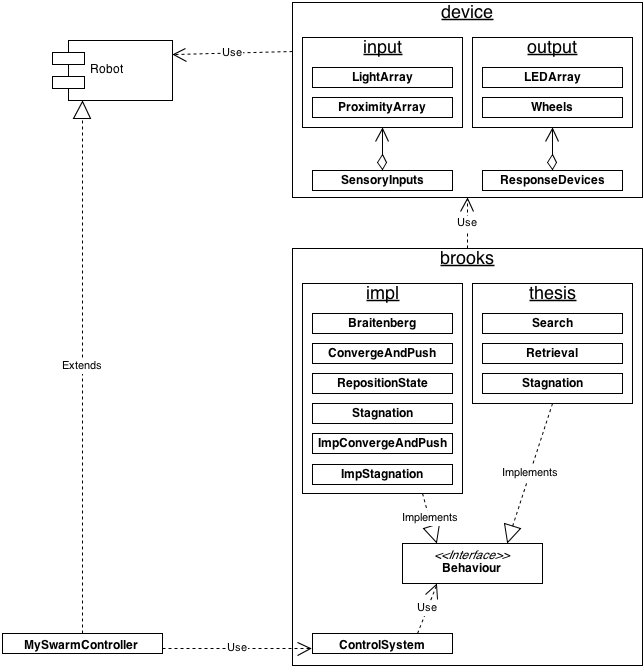
\includegraphics[width=\columnwidth]{./../images/brooksArchitecture.png}%
				\caption{Project architecture}
				\label{fig:architecture}	
			\end{figure}
			
			\shiftline In the architecture there are especially four entities worth taking a look at, 
				\textit{MySwarmController}, \textit{ControlSystem}, \textit{Behaviour} and the \textit{device} package.
			
			\shiftline \textit{MySwarmController} is the entrypoint for the controller. 
				It has the responsibility of initating the control system before start, and invoking the \textit{step} method related to webots. 
			
			\shiftline The \textit{ControlSystem} handles initialization of sub modules to be used in the subsumption architecture, 
				and the initialization of the robot abstraction. During runtime it handles invokation of submodules.
			
			\shiftline All behavioural modules implement the \textit{Behaviour} interface. This interface provide two methods, 
				\textit{trigger(SensoryInputs, ResponseDevices):Boolean} and \textit{execute(SensoryInputs, ResponseDevices):Void}. 
				The first method should check if the current world state is perceived in such a way that the module would like to be activated. 
				E.g. the random walk module will always return \textit{True}, since this is the most basic behaviour in our system. 
				The retrieval module on the other hand will check some of the input sensor, and from these make the decision. 
			
			\shiftline The \textit{device} package holds the abstraction entities used to simplify the usage of the robot, 
				and provides aggregated structures of these to minimize the amount of parameters needed to be passed through the architecture. 
				\textit{LightArray}, \textit{ProximityArray} and \textit{LEDArray} provides easy access to the light sensors, distance sensors and all the LED respectively. 
				The one who differentiate itself from the rest is \textit{Wheels}, which is an abstraction layer and extension of the provided \textit{DifferentialWheels}. 
				It was large inspirered by \textit{epuck\_basic.py}.
			
		\subsubsection{Changes to the world}
			The inital settings of the light source caused the epucks to always see the lightsource, additionally the distance to the lightsource seemed
			to have little impact on the sensor readings. Based on this we decided to change the attenuation of the lightsource from $[1,0,0]$ to $[0,0,25]$.
			This gave us the desired behaviour of the lightsource, where the epucks did not detect the source from far away and distance did affect the sensor readings.
			One downside to this change was that in close proximity of the lightsource the sensors would simply yield a zero value for the sensors facing the lightsource.
			We did however dicide to keep this change throughout the project since this effect gave us an more realistic simulation and provided us with more testing possibilities.
			
		
	\subsection{Inital implementation}
		Den klarer det...
		uforventet stacking av epucks funker greit. (De st�r bak og dytter de som er n�rmere boksen) (Implemented braitenberg search, stupidConvergeAndPush and stupidStagnationAvoidance)
		
	\subsection{Migration to thesis implementation}
		OK

\section{Part B}
	\subsection{Areas of improvement}
		\subsubsection{Architecture}
		\subsubsection{Modules}
		\subsubsection{Code}
		search: braitenburg sucks, gets stuck in corners at some times. 
		convergeAndPush: Spends a lot of time pushing when not aligned with
	the box. Move alignment from stagnation to push. 
		stagnation: Only looks directly to its side when deciding if it is going to 
	stay or not. This combined with not allways being align result in the box being counted as a neighbour in some occurences. Move alignment from stagnation to push. 
	Introduce all backwardsfacing sensors as neighboursensor, in order to also find 
	bot that are standing behind and pushing. 
		
	\subsection{Effect of improvements}
		Done
		Very well

%\pagebreak
%\tableofcontents
%\pagebreak

\end{document}